% ED-23 -- The isothermal theorem of evolutionary graph theory, kernel-checked
% English translation of papers/discovery_journal_2026/chapters/c07.tex
% Sources: TOP20.json pick 7; papers/p3_isothermal_theorem/{AUDIT.md,REVISION.md,publication_meta.json}
% Figure: code/fig07.py -> figures/c07_graphes.{pdf,png}
\chapter[The seating plan and selection]{When the seating plan changes nothing about selection}
\reference{Preprint of 26 October 2026.\\ doi:10.5281/\\zenodo.23660071}

\section*{The idea in one picture}

\begin{analogie}
A big dinner table, one chair per guest. At each round, one guest is drawn at random, with better odds if they are
``strong'' (the mutant counts $r$ times more than an ordinary guest), and they seat one of their followers on a
chair that the seating plan assigns to them, in place of its occupant. The seating plan is a network: it says who
can replace whom, and with what chance. The theorem says this: if \emph{every chair is replaced as often as the
others}, the seating plan, however twisted, changes nothing about a clan's chance of eventually occupying the whole
table. Everything happens as if the guests were well mixed.

\emph{Where the picture stops being accurate:} the result holds for this precise rule (first we choose who
reproduces, then who is replaced); with the opposite rule, or if we talk about speed rather than final chance,
nothing is proved here.
\end{analogie}

\section*{What was done}

In evolutionary theory on networks, the population sits on the vertices of a graph. A matrix $W$ gives, for each
individual $i$, the chance $W_{ij}$ that its offspring replaces individual $j$; each row of $W$ adds up to $1$. The
network is called ``isothermal'' when each column also adds up to $1$: every individual is replaced, on average, at
the same rate. The classic theorem says that then, if the network is in one piece (you can get from any vertex to
any other), the chance of taking over is exactly that of the Moran model, where the population is well mixed:
$(1-r^{-k})/(1-r^{-n})$ for $k$ mutants among $n$.

The article proves this direction of the theorem in Lean, together with a generalization where individuals receive
different reproduction weights, but ``in balance'' with the network. It reuses as is the absorption theorem of the
work on fixation probabilities (doi:10.5281/zenodo.23653850). And it begins with a confession: the formulation
announced before the work, ``the number of mutants evolves like a simple ladder'', is \emph{false} for the chain
studied. What is true, and proved, is subtler: in \emph{each} configuration, the chance of gaining a mutant is $r$
times the chance of losing one.

\begin{encadre}
\textbf{To do with a pencil.} Four guests in a circle, numbered $0,1,2,3$; each replaces one of their two
neighbours, with chance $1/2$ each. Every column adds up to $1$: the circle is isothermal. Take $r=2$ and two
mutants. The total weight is $2+2+1+1=6$.
\begin{itemize}
\item \emph{Neighbouring mutants, at 0 and 1.} To gain a mutant, either $0$ must be chosen (chance $2/6$) and aim
  at its neighbour $3$ (chance $1/2$), or $1$ must aim at $2$: $1/6+1/6=1/3$. To lose one, $2$ or $3$ must be
  chosen ($1/6$ each) and aim at the neighbouring mutant ($1/2$): $1/12+1/12=1/6$.
\item \emph{Opposite mutants, at 0 and 2.} Each mutant has only ordinary neighbours: gain $2\times2/6=2/3$,
  loss $2\times1/6=1/3$.
\end{itemize}
With the same number of mutants, the chances differ ($1/3$ or $2/3$): simple counting is not enough, hence the
error in the pre-announcement. But the gain/loss ratio is $2=r$ in both cases, and it is this ratio that gives
the formula: $(1-1/2)/(1-1/16)=8/15$ for a single mutant. Counter-test: the three-site star (a centre joined to
two leaves) is not isothermal. Its centre column adds up to $2$ and each leaf column to $1/2$: the centre is
replaced twice as often as the average, and four times as often as a leaf. A mutant placed at the centre takes
over with chance only $5/12$, instead of $4/7$; on a leaf, $2/3$; placed at random, $7/12$. These three values
are proved in Lean. Figure~\ref{fig:c07} also shows the four-site star (a centre, three leaves), where a
well-mixed population would give $8/15$: the centre takes over with only $392/1265$, a leaf with $168/253$, a
mutant placed at random with $728/1265$. Those values are only computed.
\end{encadre}

\begin{figure}[htbp]
\centering
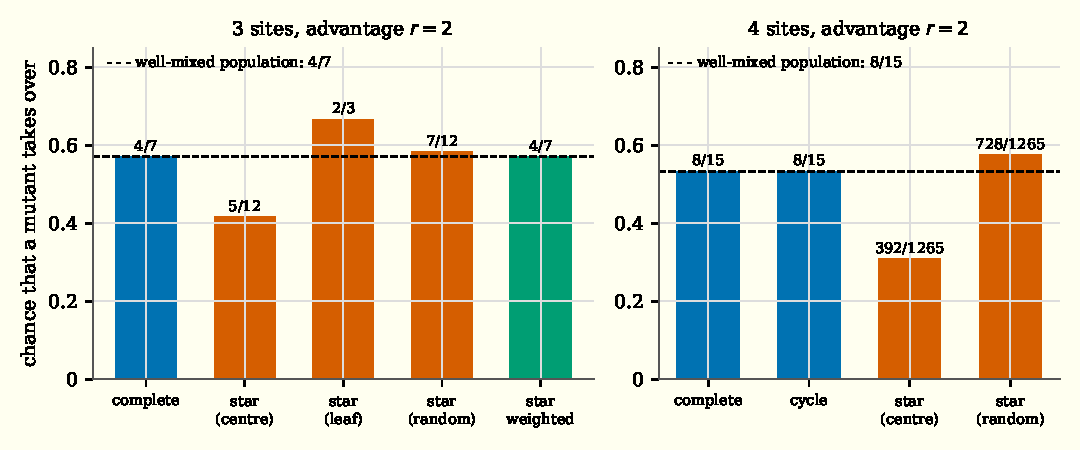
\includegraphics[width=\linewidth]{figures/c07_graphes}
\caption{Chance of invasion by a single mutant, in exact fractions, at $r=2$: on the left three sites (values proved in Lean), on the right four sites (values only computed, level~X). Isothermal networks in blue, star in orange; in green, the three-site star with weights at equilibrium, which gives back $4/7$.}
\label{fig:c07}
\end{figure}

\section*{How we made sure it is not wrong}

In short: \niveau{A} for the proved theorem and for the values of the three-site star, \niveau{C} for the
biological reading, \niveau{X} for the numerical values of the four-site star in the figure.

For the theorem, ``the judge has looked.'' The Lean kernel, the small program that checks every logical step,
accepted all the proofs, with only the three standard axioms of the whitelist. An independent auditor, an AI agent
distinct from the one that produced the work but from the same family of models, recompiled everything in its own directory, then
replayed every declaration in the kernel with a second tool: no error. It recomputed the star and the circle with
its own program in exact fractions, and found the same values.

Above all it built two false proofs, which were meant to fail. The first, with a hole plugged by \texttt{sorry},
compiles without error but the axiom audit exposes it. The second is sneakier: a debugging option that bypasses
the kernel makes it possible to ``prove'' something false, and the list of axioms then stays \emph{perfectly clean}.
Only the replay in the kernel rejected it. Lesson taken up in the corrected article: the safeguard is the list of
axioms \emph{and} the replay \emph{and} the search for these forbidden options. The register remains marked
``unaudited'': no human has yet checked that the statements say what we think they say.

\section*{What this does not say}

\begin{limite}
\begin{itemize}
\item Only the direction ``isothermal $\Rightarrow$ like a mixed population'' is proved; the converse is not.
\item Nothing about other update rules (death first, then birth), nor about weights that do not form rows adding up
  to $1$.
\item ``Chance of taking over'' here means the limit of a matrix power; the link with a law on trajectories is the
  usual definition, not formalized (\niveau{C}).
\item The values for the four-site star (figure, right) come from a Python computation in fractions, not
  verified by the kernel (\niveau{X}); those for the three-site star, by contrast, are proved in Lean.
\item No mathematical novelty is claimed: the results date from 2005, 2015 and 2024. The authors know of no earlier
  formalization, but did not do a systematic search. The biological significance (tissues, selection amplifiers)
  is an interpretation, with no data at all.
\end{itemize}
\end{limite}

\section*{Going further}

The article, the locking of the statements and the audit are deposited under doi:10.5281/\allowbreak zenodo.23660071.
It shows in a single document both reuse (it imports the building blocks of the work on fixation) and humility (it
publishes its own pre-registration error).
